% !TEX root = main.tex

\chapter{試料構造と測定方法}%================================
\section{はじめに}%========================================
本研究ではInGaAs/GaAs多重量子井戸・ファブリーペロー型の半導体レーザーをデザインした測定を行なった。本章では2.2節でそのエピ構造とデバイス化のためのプロセスについて、2.3節で測定手法について述べる。
\section{試料作製}%========================================
本研究では活性層にInGaAs/GaAs多重量子井戸を持つウエハをデザインした。本2.2節では結晶構造のデザインと測定するためのデバイス化について述べる。ウエハの結晶成長およびプロセスはNTT-ATおよびオプとウェルに依頼した。

\subsection{試料構造}%=====================================
まずはエピウエハ構造について述べる。試料は(1)3周期多重量子井戸構造と(2)10周期多重量子井戸構造のの2種類である。それぞれのエピ構造を図\ref{fig:fig_2_1_wafer_structure}に示す。
\begin{comment}
\begin{figure}[t]
	\centering
	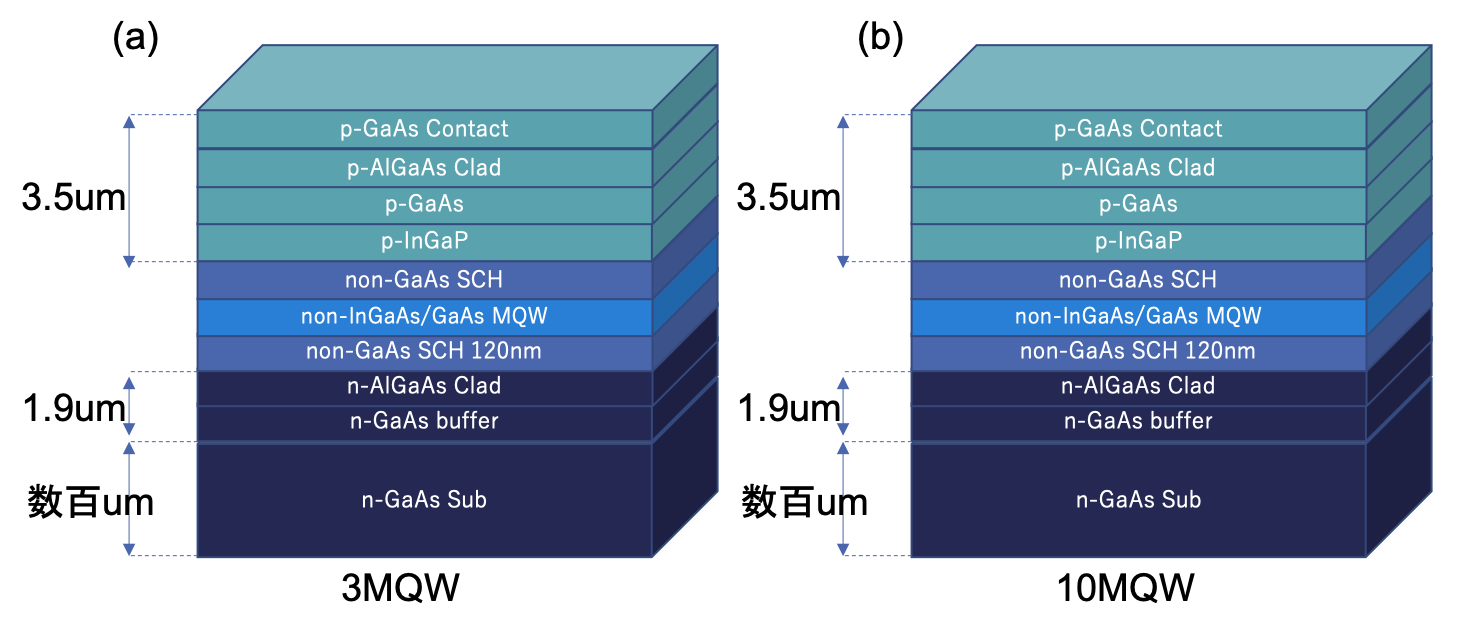
\includegraphics[width=15cm]{figure/fig_2_1_sample_structure}
	\caption{エピウエハ構造}
	\label{fig_2_1_sample_structure}
\end{figure}
\end{comment}
\begin{figure}[t]
	\centering
	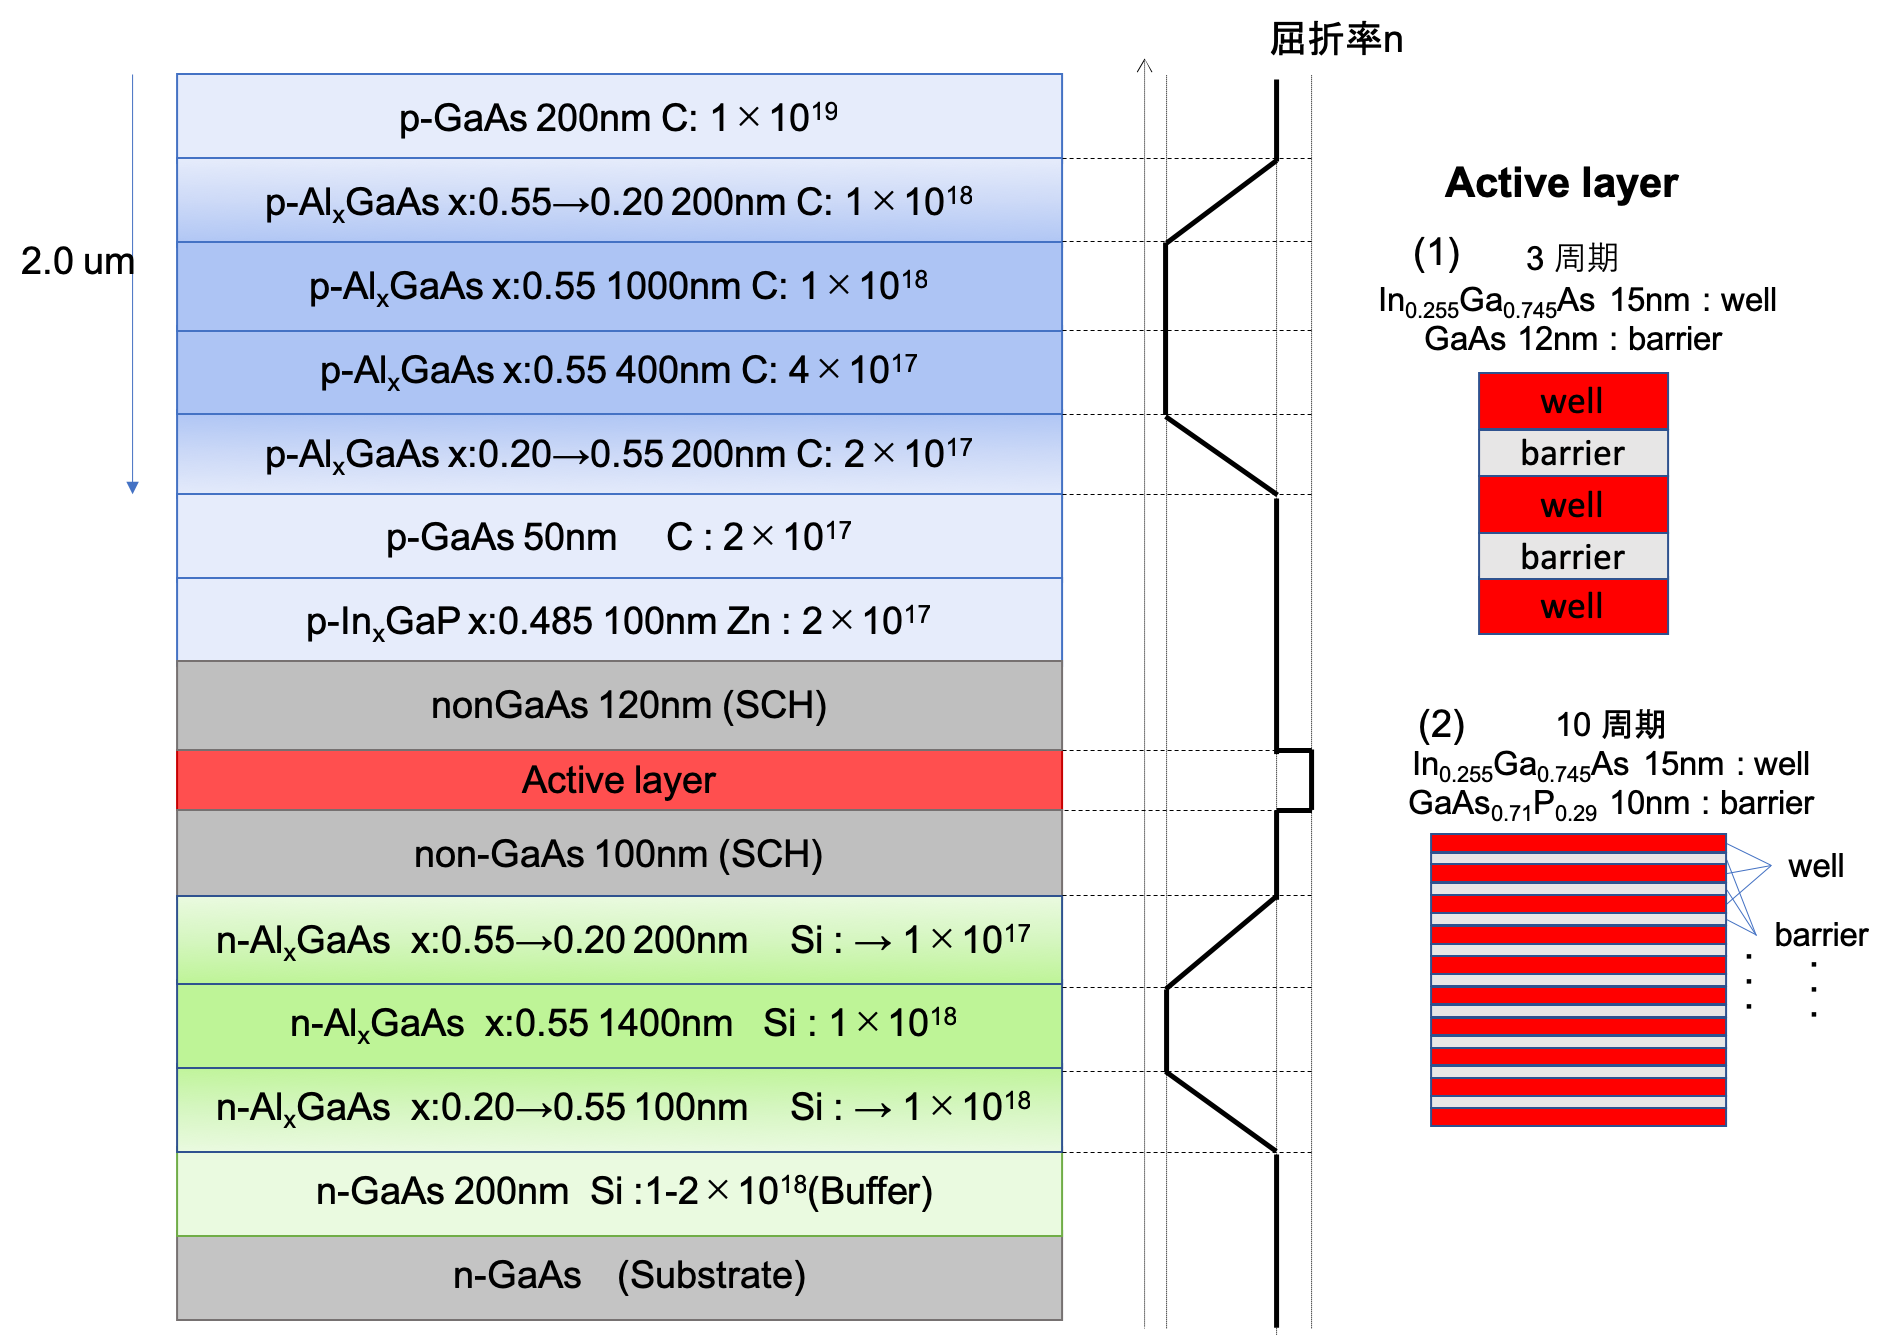
\includegraphics[width=15cm]{figure/fig_2_1_wafer_structure}
	\caption{エピウエハ構造}
	\label{fig:fig_2_1_wafer_structure}
\end{figure}
\newpage
\clearpage
\subsection{ブロードコンタクトレーザー}%=======================
ブロードコンタクトレーザーとは光導波路を形成せずコンタクト電極をベタに蒸着したレーザーである。プロセスを簡略化することで早く測定を行うことを目的とした。ウエハの評価測定のために用いた。
エピウエハのn側とp側にコンタクトメタルの蒸着を行った。p側の原子は......劈開面は001?とかなんとか
図\ref{fig:sample_broadcontact}に模式図を示す。図\ref{fig:sample_broadcontact}の上から下に向かって電流が流れ、活性層でキャリアの再結合が起き発光が起こる。また図の手前と奥の劈開面でファブリーペロー共振器を形成している。注入キャリアの量が閾値を超えると反転分布となり、光がそこを往復することで誘導放出が起きる。紙面の手前と奥方向に(z方向)共振器長はL=500,1000,2000umの3種類を作製した。また電極パッド幅はw=3,5,10,30,50,100,300umの6種類を作製した。

\begin{figure}[t]
	\centering
	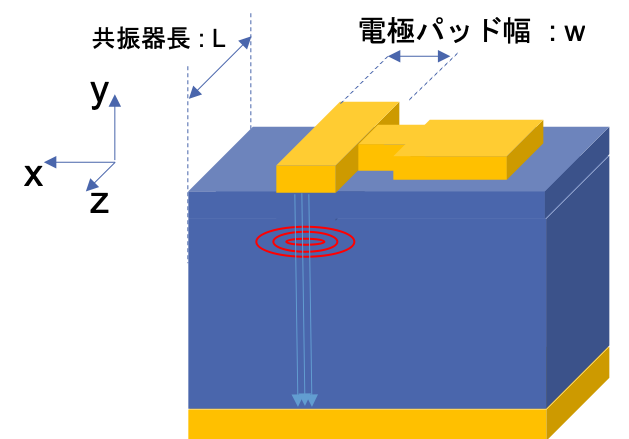
\includegraphics[width=10cm]{figure/fig_2_1_broadcontact.png}
	\caption{ブロードコンタクレーザー}
	\label{fig:sample_broadcontact}
\end{figure}

\begin{comment}
\begin{figure}[t]
	\centering
	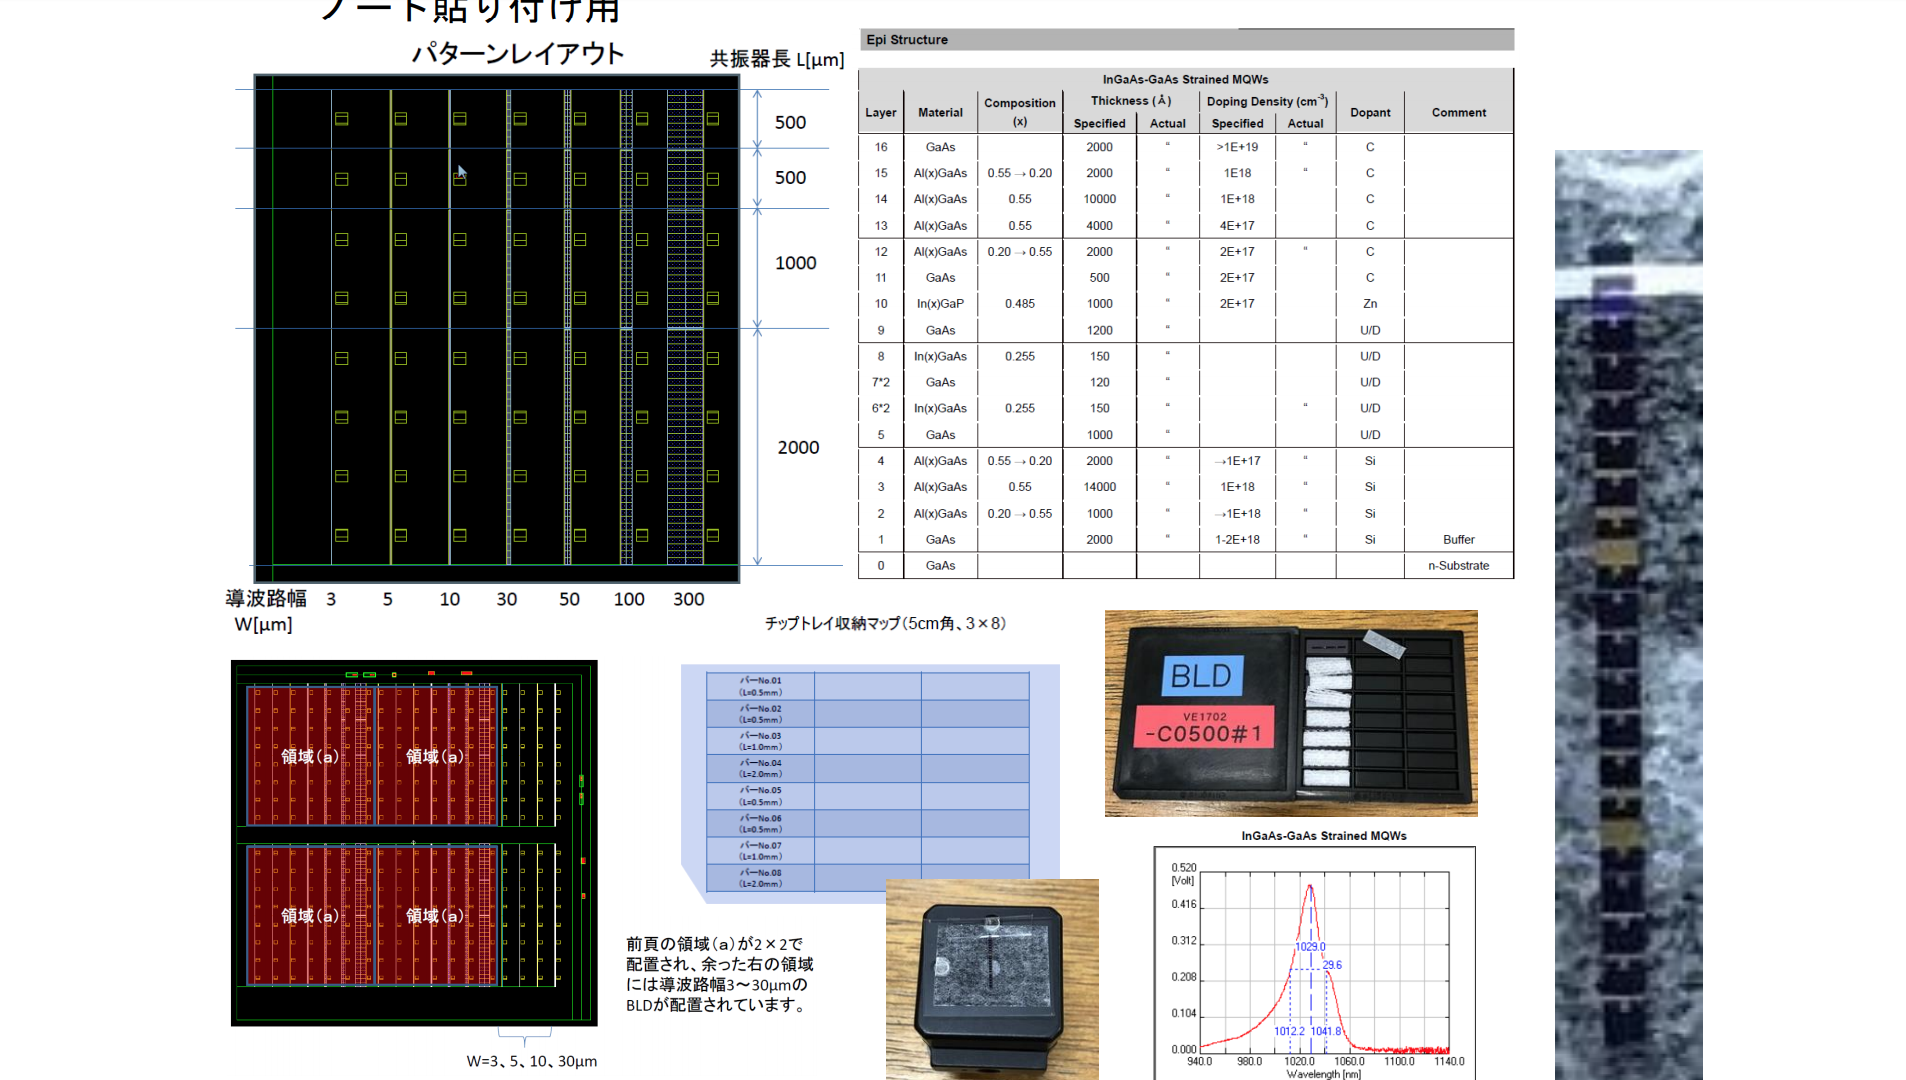
\includegraphics[width=10cm]{figure/fig_2_1_broadcontact_memo.png}
	\caption{ブロードコンタクレーザーめも}
	\label{fig:sample_broadcontact_memo}
\end{figure}
\end{comment}
\subsection{リッジ導波路型レーザー}%==========================
次にリッジ導波路型レーザーについて述べる。その模式図を図\ref{fig_2_1_ridge}に示す。エピウエハ作製後p側クラッド層を活性層直上までドライエッチングすることで光導波路を形成している。横方向(x方向)の光閉じ込めが大きくなるため、キャリアと光の重なりが大きくなることにより利得を大きくすることだできる。参考文献欲しい。一般的に行われている手法であり、本研究でも最終的に利得スイッチング動作を試みるデバイスである。
共振器長は1L=00,200,300,400,500,1000um、導波路リッジ幅はw=1.5um,2.5umのものを作製した。
リッジの深さは1.8 um(先発)と1.9$\sim$2.0um(後発)
である。
\begin{figure}[t]
	\centering
	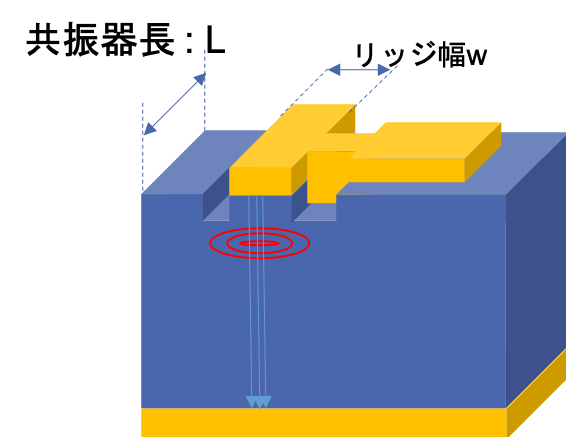
\includegraphics[width=10cm]{figure/fig_2_1_ridge.png}
	\caption{リッジ導波路型レーザー}
	\label{fig_2_1_ridge}
\end{figure}
\clearpage
\subsection{マウント(ダイボンディング??)}%======================
作製したブロードコンタクトレーザーおよびリッジ導波路型レーザーに電流注入実験を行うためにマウントを行なった。それぞれ図に示す。\\
 レーザーはAlN基板にAnSnメッキを施してあるサブマウント(....社製)にダイボンディングを行った。
ブロードコンタクトレーザーはダイボンディングしてなかったっけ?そういえば
この状態で試料上面の電極をプローバー(先端の径...程度の金属の針)でさわり、電流を流した。一本のバーに5から6個程度の素子があるので測定が終わったら次々とプローバーの触る箇所をかえていけば速やかに測定を続けることができる。\\
 一方、利得スイッチング動作実験を行う試料は短い電気パルスが入るようにTransistor Outlineパッケージと呼ばれる缶状の金属にマウントを行った。....社製のCANを用いた。分離した素子をAnSn共晶材あるいはエポキシを用いてCANにダイボンディングし、金線をワイヤーボンディングマシンで配線した。その例を図\ref{fig:fig_2_1_mount_GS}に示す。


\begin{figure}[h]
	\centering
	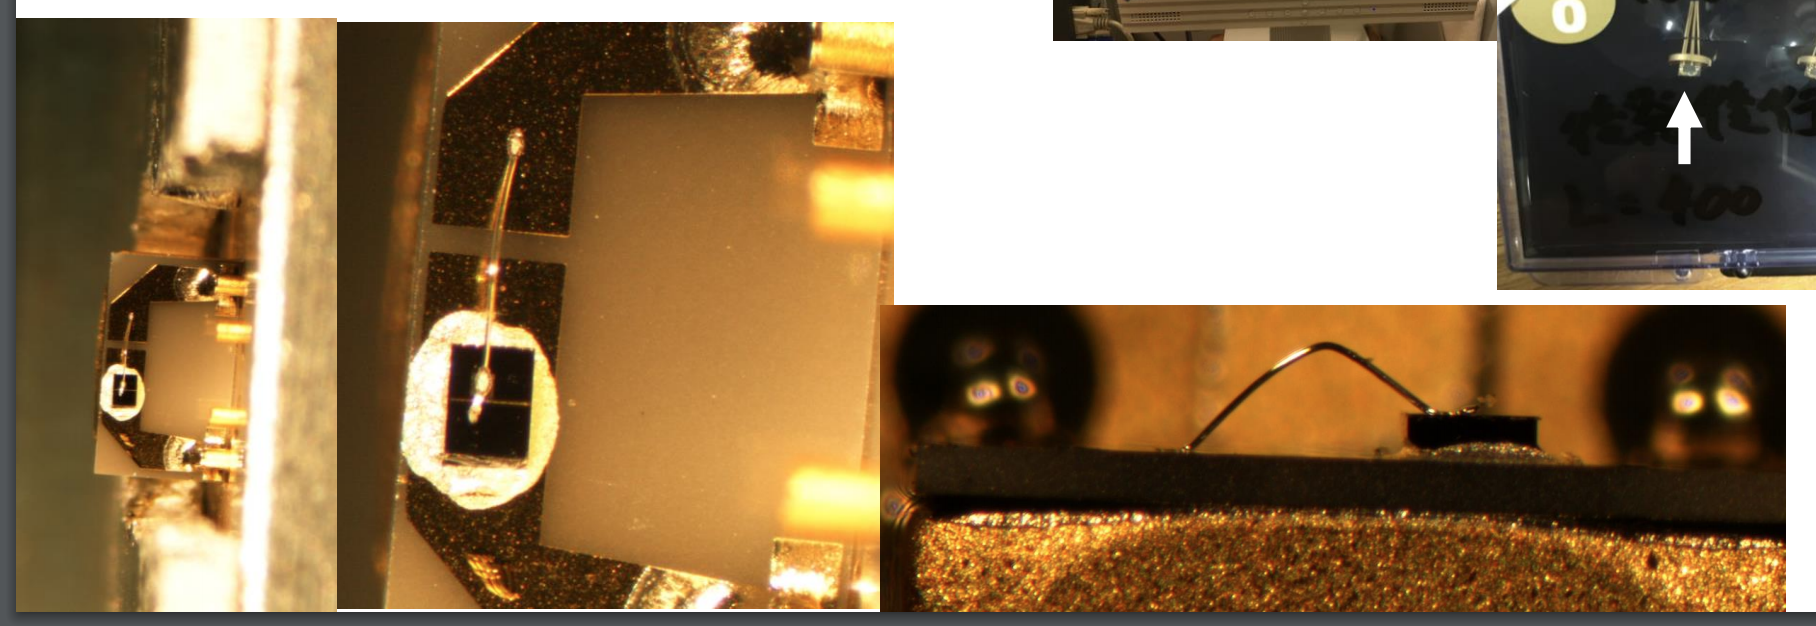
\includegraphics[width=15cm]{figure/fig_2_1_mount.png}
	\caption{利得スイッチング測定デバイス外観}
	\label{fig:fig_2_1_mount_GS}
\end{figure}
\clearpage
\section{測定方法}%========================================
本研究では主に2つの実験を行った。1つはエピウエハの品質を評価するための定常電流を印加する実験である。もう一つは利得スイッチング動作を起こすための短い電気パルスを印加する実験である。それぞれについて2.3.1節と2.3.2節で述べる。
\subsection{定常電流注入による測定実験}%=======================
まずエピウエハの品質を調べるために定常電流を注入する実験である。発振閾値電流や発振時の発光効率すなわち外部量子効率などの基本的な物性パラメータを見積もることができる。
実験系を図\ref{fig:fig_2_2_IL_setup}に示す。パルスジェネレータから数usパルスを数ms繰り返し周期で発生させ試料に注入する。ここでマイクロ秒程度のパルスは試料の中での発光過程やその他の物理現象の時間オーダーに対して十分長く、定常電流とみなすことができる。DC電流では熱の影響が大きくなってしまい試料が壊れてしまう恐れがあるため。Duty比(パルス幅と繰り返し周期の比)を1:1000程度に設定して実験を行った。試料からの発光強度を光パワーメータで測定した。また、回路に試料と直列に抵抗(22.4$\rm{\Omega}$)を入れ、そこにかかる電圧をモニタすることで流れる電流をそくていした。また回路全体の電圧と抵抗にかかる電圧の差をとることで試料にかかる電圧を算出した。

本来であればDC電流を印可することで定常発振させることが望ましい。しかし試料への熱の影響が無視できないほど大きくなってしまうため、本研究ではDC電流の代わりにマイクロ秒程度パルス電圧を印可した。マイクロ秒は半導体素子の中が定常状態になるには十分長く印可している時間の間に定常発振が起きているものとみなしていること。

\begin{figure}[htbp]
	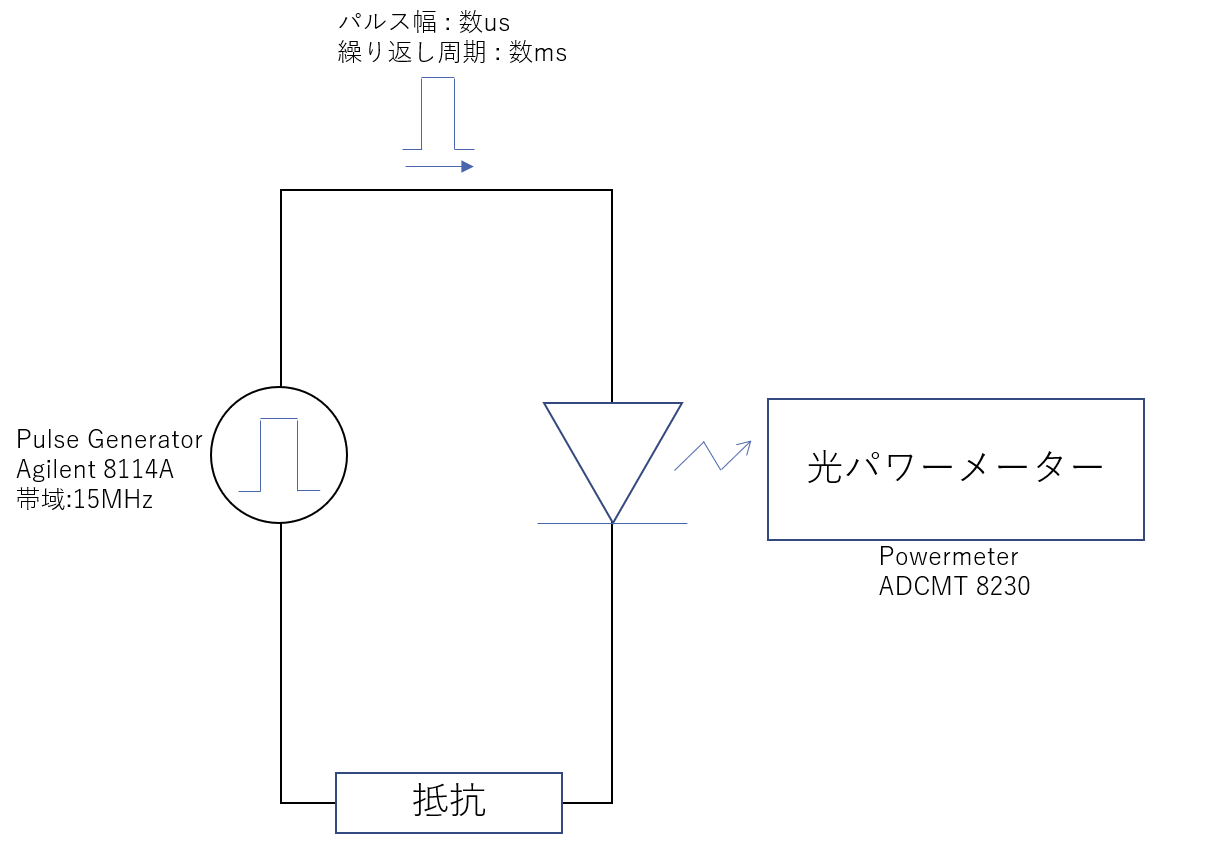
\includegraphics[width=15cm]{figure/fig_2_2_IL_setup.png}
	\caption{定常電流注入実験の実験系回路図}
	\label{fig:fig_2_2_IL_setup}
\end{figure}
\clearpage
ここで用いた機材を\ref{table:table_2_2_IL_setup}に示す。
\begin{table}[hbtp]
  \caption{定常電流印加実験に用いた機材}
  \label{table:table_2_2_IL_setup}
  \centering
  \begin{tabular}{lcr}
    \hline
    機材  & 型番     \\
    \hline \hline
    Pulse Generator  & Agilent 8114A   \\
    Power Meter  &  ADCMT 8230    \\
    Oscilloscope  &  埋める  \\
       \hline
  \end{tabular}
\end{table}
 \clearpage
\subsection{電流注入利得スイッチング実験}%======================
ナノ秒程度の短いパルス電圧を印加することで利得スイッチング動作を起こした。その実験系の回路図を図\ref{fig:fig_2_3_GS_setup}。電気パルスがパルスジェネレータから同軸ケーブルを介して試料へ印加される。パルスジェネレータで生成された電圧パルスは可変抵抗、RFアンプで増幅されデバイスへと印可される。試料からの発光は対物レンズでコリメートされ、非球面レンズで光ファイバーに集光される。その後フォトダイオードで検出しその電圧を高速サンプリングオシロスコープでモニタすることで光の時間波形を測定した。
\begin{figure}[htbp]
	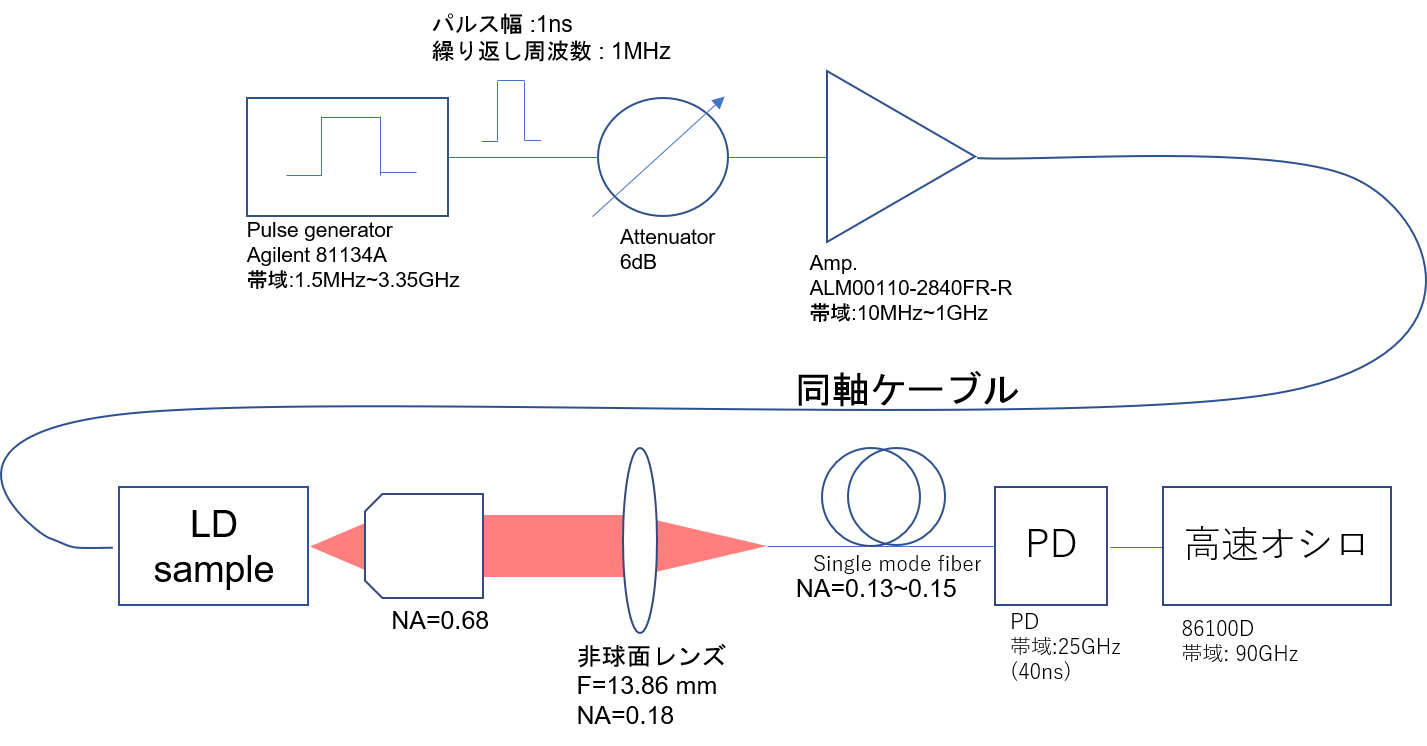
\includegraphics[width=15cm]{figure/fig_2_3_GS_setup.png}
	\caption{GS実験系}
	\label{fig:fig_2_3_GS_setup}
\end{figure}
この実験で用いた機材を表\ref{table:table_2_2_GS_setup}にまとめた。
\begin{table}[hbtp]
  \caption{利得スイッチング実験に用いた機材}
  \label{table:table_2_2_GS_setup}
  \centering
  \begin{tabular}{lcr}
    \hline
    機材  & 型番   & 帯域  \\
    \hline \hline
    Pulse Generator  & Agilent 81143A & 1.5MHz$\sim$ 3.35GHz   \\
    Atteuator  &  埋める    & 埋める\\
    RF Amp & ALM00110-2840FR-R & 10MHz $\sim$ 1GHz \\
    PD & 埋める & 25GHz \\
    Oscilloscope  &  86100D & 90GHz  \\
       \hline
  \end{tabular}
\end{table}
